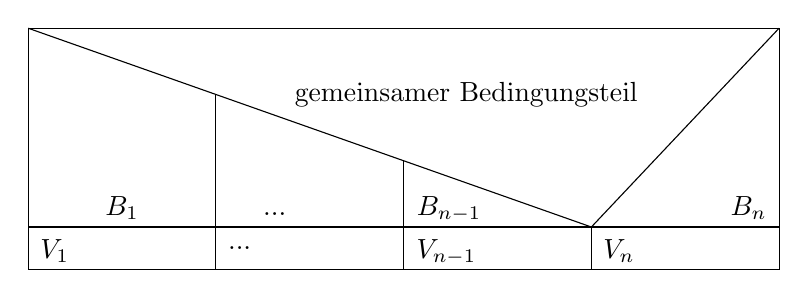
\begin{tikzpicture}
    \draw (0pt,0pt) rectangle (271.31702pt, -71.83336pt);
    \node at (4.0pt, -35.91668pt) {};
    \draw (0pt, 0pt) -- (203.48776500000002pt, -71.83336pt);
    \draw (203.48776500000002pt, -71.83336pt) -- (271.31702pt, 0pt);
    \draw (67.829255pt, -23.944453333333332pt) -- (67.829255pt, -71.83336pt);
    \draw (135.65851pt, -47.888906666666664pt) -- (135.65851pt, -71.83336pt);
    \node at (33.9146275pt, -64.913365pt) {$B_1$};
    \node at (89.06782375pt, -67.25545pt) {$...$};
    \node at (152.07071000000002pt, -65.33005pt) {$B_{n-1}$};
    \node at (260.335455pt, -64.913365pt) {$B_n$};
    \node at (158.2682616666667pt, -23.944453333333332pt) {gemeinsamer Bedingungsteil};
    \draw (0pt,-71.83336pt) rectangle (67.829255pt, -87.31584pt);
    \node at (9.56878pt, -80.39584500000001pt) {$V_1$};
    \draw (67.829255pt,-71.83336pt) rectangle (135.65851pt, -87.31584pt);
    \node at (76.391765pt, -79.5746pt) {$...$};
    \draw (135.65851pt,-71.83336pt) rectangle (203.48776500000002pt, -87.31584pt);
    \node at (151.111625pt, -80.81253000000001pt) {$V_{n-1}$};
    \draw (203.48776500000002pt,-71.83336pt) rectangle (271.31702pt, -87.31584pt);
    \node at (213.51025pt, -80.39584500000001pt) {$V_n$};
\end{tikzpicture}
